We use a Bayesian approach to model comparison to find out which model
best explains the data described in the previous section
\cite{VandekerckhoveMatzke2013:Model-Compariso}. The models under
investigation have unspecified parameters: the speaker's degree of of
rationality $\lambda_\mathrm{S}$, the cost of adjectives $c$, and, for
those listener models that have an action-oriented communication goal
, the listener's degree of rationality $\lambda_\mathrm{L}$. Since
there is no principled theory to determine the value of the
parameters, we will rely on relatively uninformed hyperpriors
(so-called to distinguish them from the salience priors). Based on a
specification of hyperpriors, we calculate the models' \emph{evidence}
and compare them by their \emph{Bayes factors}. The evidence of a
model $M$ is the weighted average of the likelihood of observing the
data under all parameter values:
\begin{align}
  \label{BMA}
  \mathrm{Ev}(M)= \int \Pr(\theta) \cdot p(D | M, \theta)\, \mathrm{d}\theta,
\end{align}
where $\Pr(\theta)$ is the hyperprior over parameter(-tuple) $\theta$
associated with $M$ and $D$ is the observed data. The Bayes factor
$K^{M_1}_{M_2}$ is a comparative measure for the plausibility of model
$M_1$ over $M_2$, given their respective hyperpriors and the data in
question:
\begin{align}
  K^{M_1}_{M_2} = \frac{\mathrm{Ev}(M_1)}{\mathrm{Ev}(M_2)} \enspace .
\end{align}
Model $M_1$ makes the data more likely whenever $K^{M_1}_{M_2}$, but
normally only a Bayes factor $K^{M_1}_{M_2} >3$ (or sometimes
$K^{M_1}_{M_2} > 5$) is considered substantial. Values $K^{M_1}_{M_2}
> 10$ are considered strong evidence.

In a sense, comparison by Bayes factors is comparing models in a wider
sense of the term: we actually compare pairs consisting of a model and
its associated hyperprior. For clarity, we refer henceforth to a
model-hyperprior pair as a Model.

First we look at the speaker models $\sigma_{xy},\
x\in\{a,b\},y\in\{\mathcal{U},\mathcal{S}\}$. Each model has two
parameters $\lambda_\mathrm{S}$ and $c$. We assume that they are
independent of each other:
\begin{equation}\label{hyper-speaker-independent}
\Pr(\lambda_\mathrm{S},c)=\Pr(\lambda_\mathrm{S}) \cdot \Pr(c) \enspace .
\end{equation}
We are uncertain about the rationality of the speaker:
\begin{equation}\label{hyper-speaker-lambda}
\Pr(\lambda_\mathrm{S})= \mathcal{U}_{(0,11)}(\lambda_\mathrm{S}),
\end{equation}
which is a uniform distribution over $(0,11)$. Excluding
$\lambda$-values $\ge 11$ serves practical purposes only, but is
innocuous since the regions of maximum a posteriori likelihood of
$\lambda$ lies safely in the chosen interval for all models. Next, to
allow for the possibility of speaker preferences (nouns over
adjectives or vice versa), we consider two types of hyperpriors for
costs $c$. The first hyperprior has $c=0$ with probability $1$, which
captures the assumption that there is no speaker preference. The
second hyperprior is $\mathcal{U}_{(-0.4,0.4)}$, which captures the
notion that a preference exists, without commitment to either
direction. We restrict our attention to the interval $(-0.4,0.4)$,
because we consider higher levels of cost implausible, given that
utilities for successful communication live in $[0,1]$ and that we
believe that strive for communicative success should outrank
preference satisfaction in a rational model of communication. Taken
together, there are four speaker models, two hyperpriors for each, so
that we compare eight Models with respect to their evidences.

Evidences of speaker Models were calculated by grid approximation. The
results are shown in Table \ref{table:speaker mod}. We can see
\todo{include hinton diagrams?} that the data very strongly supports
speaker models that do not take the listener's perceptual salience
into account. Also, it seems that action-oriented models are slightly
better than their belief-oriented counterparts, even though the
relevant Bayes factors are not substantial by common
standards. Finally, our data makes each speaker Model that does allow
for a speaker preference strongly more plausible than its
counterpart that does not. A look at the posterior likelihood of $c$
for each speaker model informs us that our data supports the belief
that the speakers have a preference for nouns, see
Figure~\ref{fig:cost_post_s}. \todo{improve plot}
%
\begin{table}[htb] 
  \centering 
  \caption{Evidences of speaker Models}
  \begin{tabular}{lcccc}
    support of $P(c)$ 
    & $\sigma_{\mathrm{b}\mathcal{U}}$
    & $\sigma_{\mathrm{a}\mathcal{U}}$
    & $\sigma_{\mathrm{b}\mathcal{S}}$
    & $\sigma_{\mathrm{a}\mathcal{S}}$
    \\ \midrule
    $[0,0]$
    & 4.93e-30
    & 3.56e-30
    & 5.92e-46
    & 3.09e-69
    \\
    $(-0.4,0.4)$
    & 5.04e-15
    & 4.02e-15
    & 4.28e-36
    & 3.27e-61
  \end{tabular} 
  \label{table:speaker mod}
\end{table}
%
\begin{figure}[htb]
  \centering
  \caption{Posterior distributions over costs given the data for each
    speaker model.}
  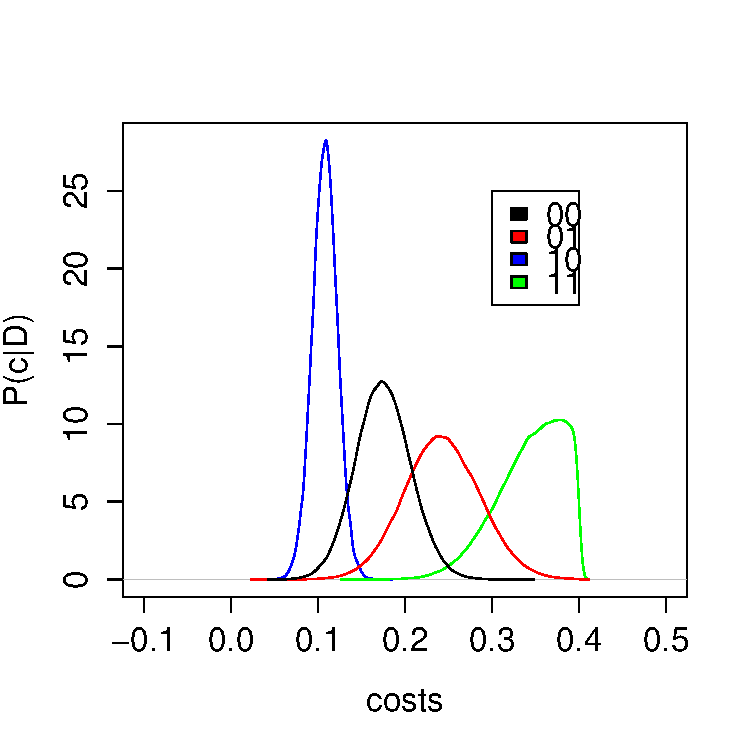
\includegraphics[width=0.5\textwidth]{pics/cost_post_s.pdf}
  \label{fig:cost_post_s}
\end{figure}
%
In sum, our data supports the belief that the speaker does not take
into account the preceptual salience of the listener, while having her
own preference for shape terms over color terms.


Now we compare the listener models, each of which has a speaker model nested inside as the belief of the listener. Since we want to know how such a belief correlates with the actual production, we put two kinds of hyperpriors under investigation. On the one hand, the flat-independent hyperpriors treat different parameters as  independent:
\begin{equation}\label{hyper-listener-independent}
\Pr(\lambda_\mathrm{S},c,\lambda_\mathrm{L})=\mathcal{U}_{(0,11)}(\lambda_\mathrm{S}) \cdot \Pr(c) \cdot  \mathcal{U}_{(0,11)}( \lambda_\mathrm{L}) \enspace .
\end{equation}
On the other hand, the true-correlated hyperpriors use the data from the speaker condition to estimate the hyperpriors for $\lambda_\mathrm{S}$ and $c$, and let $\lambda_\mathrm{L}$ have the same distribution as $\lambda_\mathrm{S}$:
\begin{equation}\label{hyper-listener-independent}
\Pr(\lambda_\mathrm{S},c,\lambda_\mathrm{L})=\mathcal{U}_{(0,11)}(\lambda_\mathrm{S} \mid D_\mathrm{S}, M_\mathrm{S}) \,\Pr(c\mid D_\mathrm{S}, M_\mathrm{S})  \,\mathcal{U}_{(0,11)}( \lambda_\mathrm{L} \mid D_\mathrm{S}, M_\mathrm{S}),
\end{equation}
and thus put a stronger constraint on the listener's belief about the speaker. 

The comparison result of the speaker models are shown in Table \ref{table:listener mod}. The best model, which is substantially better than the rest, is action-oriented and takes perceptual salience into account. It has a true-correlated speaker model which is action-oriented and does not take perceptual salience nor speaker preference into account. Note that the nested speaker model is different from the best actual speaker model only in that it does not incorporate speaker preference.  

\begin{table}[htb] 
\caption{Listener Model Comparison}
  \centering 
  \begin{tabular}{ccccc}
    rank
    & model
    & hyperprior
    & sp.~pref.
    & evidence 
    \\ \hline
    1 
    & $\rho_{\mathrm{a}\mathcal{S}}(\sigma_{\mathrm{a}\mathcal{U}})$
    & true correlated
    & $-$
    & 1.11E-003
    \\ \\
    2 
    & $\rho_{\mathrm{ a}\mathcal{S}}(\sigma_{\mathrm{b}\mathcal{U}})$
    & true correlated
    & $-$
    & 2.36E-004
    \\     
    3 
    & $\rho_{\mathrm{b}\mathcal{U}}(\sigma_{\mathrm{b}\mathcal{S}})$
    & flat independent \quad
    & adj.~or nouns \quad
    & 1.29E-004
    \\     
    4 
    & $\rho_{\mathrm{a}\mathcal{U}}(\sigma_{\mathrm{b}\mathcal{S}})$
    & flat independent
    & none
    & 9.94E-005
    \\     
    5 
    & $\rho_{\mathrm{a}\mathcal{U}}(\sigma_{\mathrm{b}\mathcal{S}})$
    & flat independent
    & adj.~or nouns
    & 8.79E-005
    \\
    $\vdots$\\
    14 
    & $\rho_{\mathrm{b}\mathcal{S}}(\sigma_{\mathrm{b}\mathcal{U}})$
    & flat independent
    & adj.~or nouns
    & 5.31E-005
    \\
    $\vdots$\\
    19 
    & $\rho_{\mathrm{b}\mathcal{S}}(\sigma_{\mathrm{b}\mathcal{U}})$
    & true correlated
    & $-$
    & 2.91E-005
    \\
    $\vdots$
  \end{tabular}
  \label{table:listener mod}
\end{table}

Combining the model comparison results for both the speaker and the listener models, it seems that if we treat the speaker's preference as some lexical salience which together with the listener's perceptual salience constitutes the contextual salience of the referential game, then contextual salience actually manifests \emph{lack of} common knowledge between the speaker and the listener rather than the presence of it, since they both have some preference that biases their decisions but they are unaware of each other's such preference. However, there is indeed something common between the speaker and the listener, i.e. the distribution of the degree of rationality. Also, the listener's belief about the speaker is correct modulo the speaker's private lexical salience. 


%%% Local Variables: 
%%% mode: latex
%%% TeX-master: "main"
%%% TeX-PDF-mode: t
%%% End: